% !TEX root = ../Thesis.tex
\chapter{Body of the Thesis}

This is the body of the thesis.

\section{Structure}
\label{sec:my-label}

\subsection{Sub-Section}

\subsubsection{Sub-Sub-Section}

\paragraph{Paragraph}

\subparagraph{Even Sub-Paragraph}

This is the body text. Make sure that when you reference anything you use labels and references. When you refer to anything, you normally capitalise the type of object you reference to, e.g. Section~\ref{sec:my-label} instead of section~\ref{sec:my-label}. You may also just use the \texttt{cref} command and it will generate the label, e.g., for \cref{sec:my-label}, we did not specify the word ``Section''.

Hint: Try to structure your labels as it is done with \texttt{sec:my-label} and \texttt{fig:machine}, etc.



\section{Equations}
A Turing Machine is a 7-Tuple:
\begin{equation}
    M = \langle Q, \Gamma, b, \Sigma, \delta, q_0, F \rangle
\end{equation}
A Turing Machine is a 7-Tuple even if defined in the text, as in $M = \langle Q, \Gamma, b, \Sigma, \delta, q_0, F \rangle$.




\section{Tables}
Some tables can also be used as shown in Table~\ref{tab:table}\footnote{Table captions are normally above the table.}. Remember that tables might be positioned elsewhere in the document. You can force positioning by putting a \texttt{ht!} in the definition.

\begin{table}[ht!]
\centering
\caption{Frequency of Paper Citations. By the way: Make sure to put the label always after the caption, otherwise \LaTeX{} might reference wrongly!}
\begin{tabular}{lcl} \toprule
Title&$f$&Comments\\ \midrule
The chemical basis of morphogenesis & 7327 & \\ 
On computable numbers, with an application to the ... & 6347 & Turing Machine\\
Computing machinery and intelligence & 6130 & \\ \bottomrule
\end{tabular}
\label{tab:table}
\end{table}




\section{Figures}
Figures are nice to show concepts visually. For organising well your thesis, put all figures in the Figures folder. Figure~\ref{fig:machine} shows how to insert an image into your document. Figure~\ref{fig:tm} references a figure with multiple sub-figures. \todoMissing{Description of figure.}

\begin{figure}
\centering
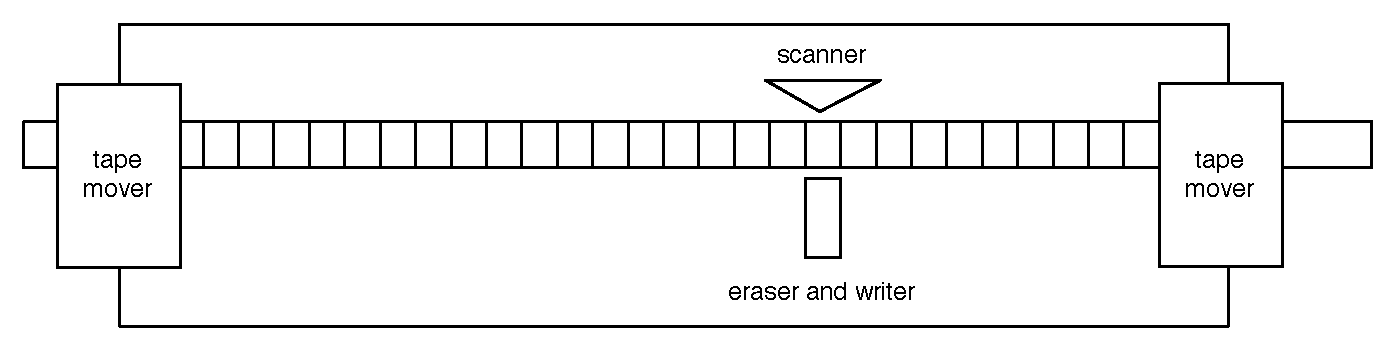
\includegraphics[width=0.9\textwidth]{turingmachine}
\caption{A Turing machine.}
\label{fig:machine}
\end{figure}


\begin{figure}
\centering
\subbottom[Turing Machine 1]{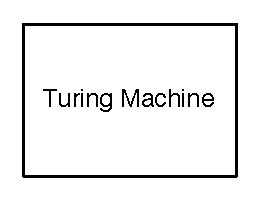
\includegraphics[width=0.2\textwidth]{block}\label{fig:tm:tm1}}
\subbottom[Turing Machine 2]{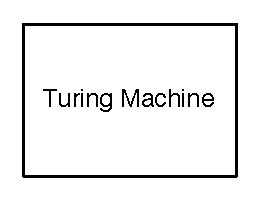
\includegraphics[width=0.2\textwidth]{block}\label{fig:tm:tm2}}
\subbottom[Turing Machine 3]{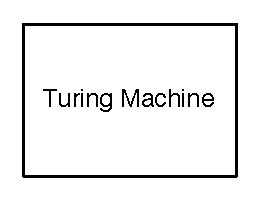
\includegraphics[width=0.2\textwidth]{block}\label{fig:tm:tm3}}
\subbottom[Turing Machine 4]{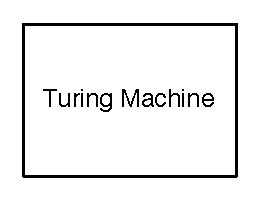
\includegraphics[width=0.2\textwidth]{block}\label{fig:tm:tm4}}
\caption{Plots of four Turing machines}
\label{fig:tm}
\end{figure}




\section{Packages}
These packages might be helpful for writing your thesis:

\begin{description}
	\item[\texttt{caption}] to adjust the look of your captions
	\item[\texttt{glossaries}] for creating glossaries (also list of symbols)
	\item[\texttt{makeidx}] for indexes and the back of your document
	\item[\texttt{algorithm, algorithmicx, algpseudocode}] for adding algorithms to your document
\end{description}